\chapter{Theorie} \label{chap:graph_theory}

In der Theorie werden die notwendigen Begriffe, die topologischen Indizes sowie ein bisheriger Ansatz zur Graphenklassifikation und Usefulness beschrieben.
Es werden Grundlagen der Graphentheorie sowie aktuelle Forschungsergebnisse vorgestellt.

Die Graphenklassen, welche in der Arbeit verwendet werden, sind in Kapitel \ref{sec:graph_classes} beschrieben.

\newpage

\section{Was ist Graphentheorie?}

Die Graphentheorie ist ein Zweig der Mathematik, der mit der Untersuchung von Graphen befasst ist, wobei es sich um Strukturen handelt, die aus Knoten (eng. Nodes, auch Punkte genannt) und Kanten (eng. Edges, auch Bögen oder Linien genannt) bestehen, die die Knoten verbinden.
Graphen sind ein nützliches Werkzeug zum Modellieren und Verstehen der Beziehungen zwischen verschiedenen Objekten oder Entitäten und sie haben zahlreiche Anwendungen in einer Vielzahl von Bereichen,
darunter Informatik, Ingenieurwesen, Biologie und Soziologie \cite[p.~1ff.]{bollobas_modern_1998}.

Auf Abbildung \ref{fig:overview_indices} folgt eine Übersicht, in welcher die Arbeit verschiedenen Feldern der Lehre und Forschung angegliedert wird.
Sie zeigt Schnittstellen zu diversen Bereichen und gibt den Zusammenhang der topologischen Indizes zu anderen Themen wieder.

\begin{figure}[H]
    \centering
    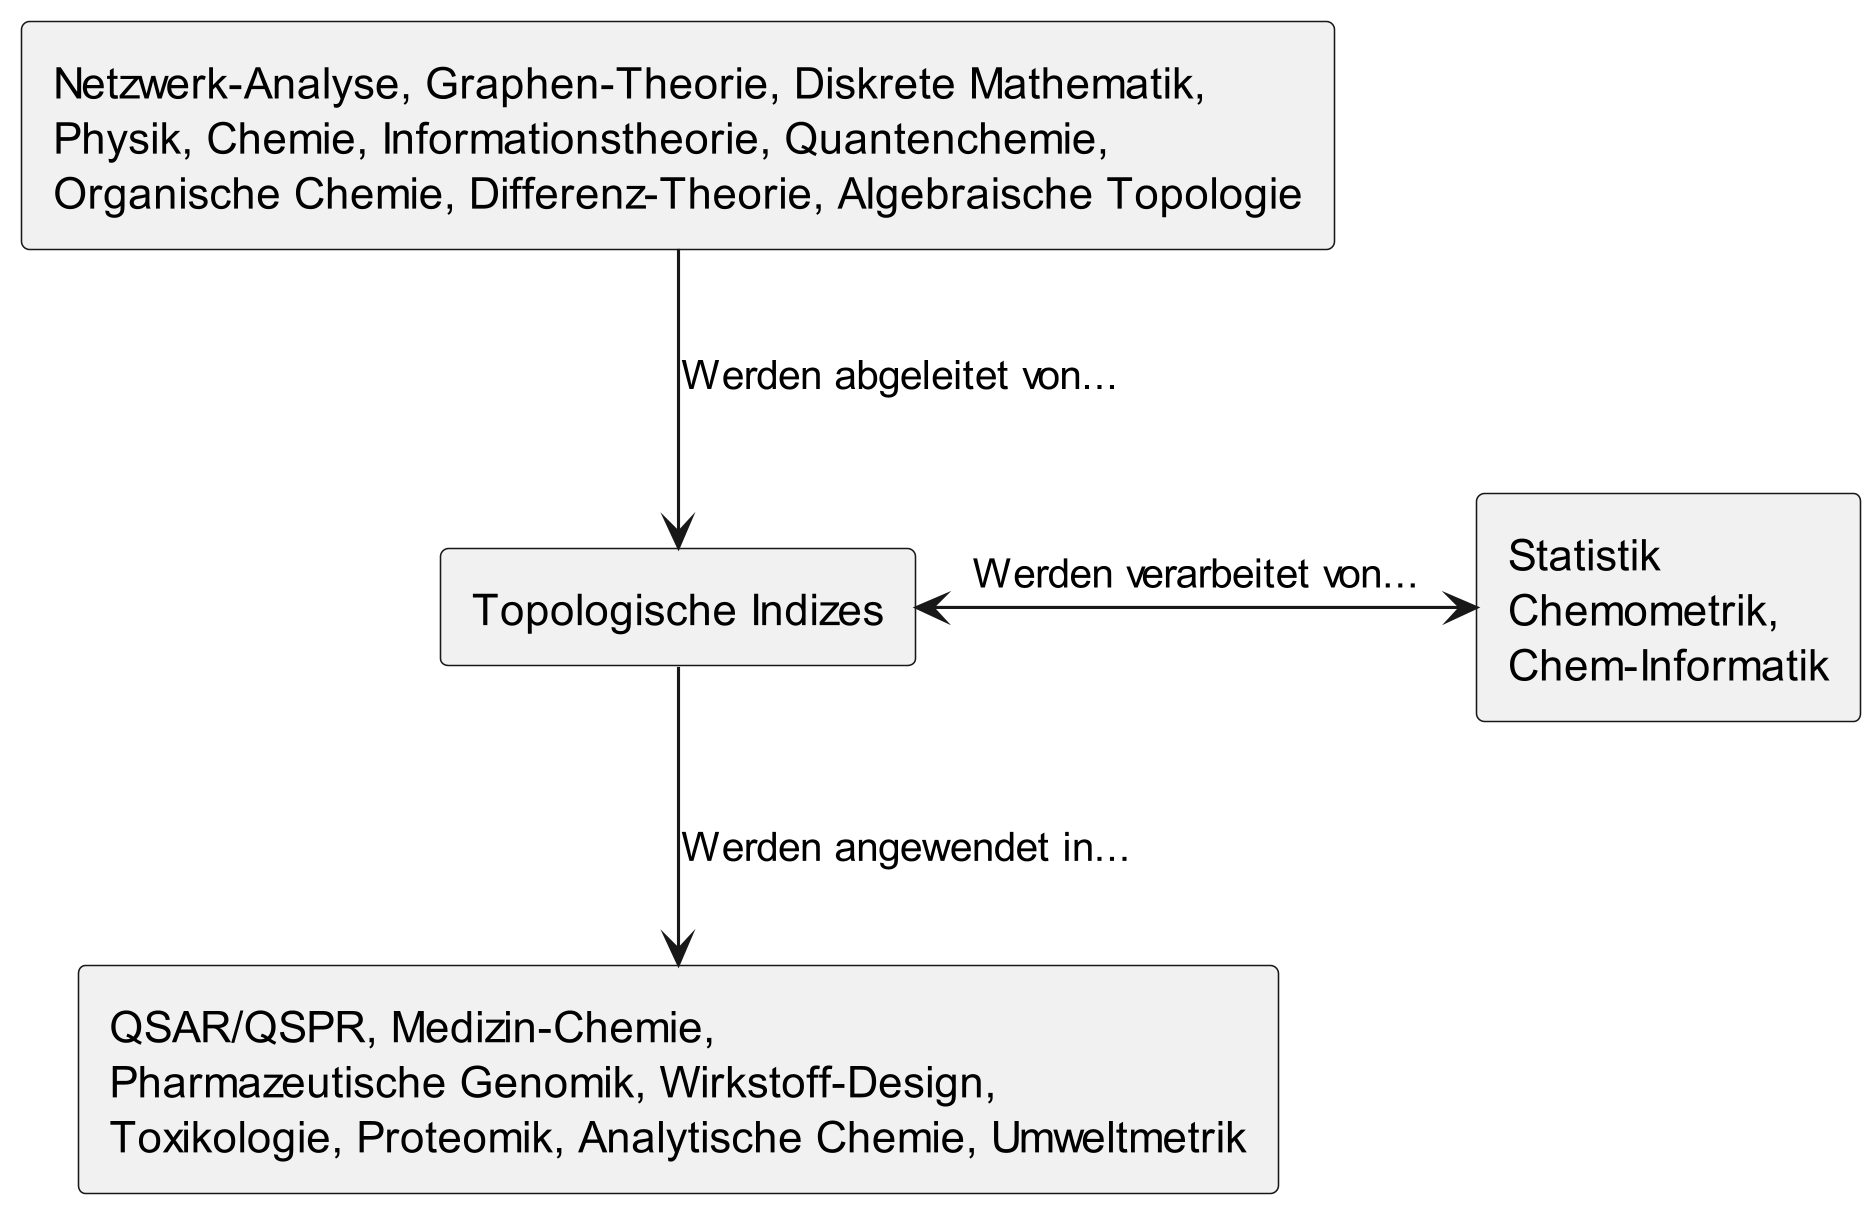
\includegraphics[width=0.9\textwidth]{images/10_introduction/overview_molecule_descriptor.png}
    \caption{Übersicht zur Anordnung des Themengebietes, übersetzt aus Todeschini und Consonni \cite{todeschini_handbook_2000}}
    \label{fig:overview_indices}
\end{figure}

Eine der Hauptanwendungen der Graphentheorie ist die Darstellung und Analyse von Netzwerken.
Beispielsweise kann ein soziales Netzwerk als Graph dargestellt werden, mit Menschen als Knoten und den Beziehungen zwischen ihnen (Freundschaften, familiäre Bindungen etc.) als Kanten.
Die Analyse der Struktur des Netzwerks kann Aufschluss darüber geben, wie sich Informationen im Netzwerk verbreiten und welche Faktoren die Veränderung des Netzwerks beeinflussen können \cite[p.~440ff.]{watts_collective_1998}.

Die Graphentheorie wird auch dazu verwendet, Probleme in der Informatik und den Ingenieurwissenschaften zu lösen.
Sie kann etwa genutzt werden, um den kürzesten Weg zwischen zwei Punkten in einem Verkehrsnetz zu finden \cite[p.~269]{dijkstra_note_1959} oder um Aufgaben in einem Computersystem zu planen \cite[p.~9]{garey_computers_1990}.
In der Biologie kann die Graphentheorie eingesetzt werden, um die Wechselwirkungen zwischen Genen oder Proteinen in einer Zelle zu untersuchen \cite[p.~3]{albert_diameter_1999} und in der Soziologie, um die Struktur sozialer Netzwerke und deren Kommunikationsmuster zu analysieren \cite[p.~1ff.]{barnes_graph_1969}.

\section{Was ist ein Graph?}

Formell wird ein Graph als $G = (V, E)$ definiert, wobei $V$ die Menge der Knoten und $E$ die Menge der Kanten ist.
Knoten können als Punkte oder Kreise dargestellt werden und Kanten als Linien, die zwei Knoten verbinden \cite[p.~45]{barabasi_network_2016}.

Ein Graph kann \textbf{\textit{ungerichtet}} oder \textbf{\textit{gerichtet}} sein. Bei einem ungerichteten Graphen können die Kanten in beide Richtungen durchlaufen werden.
Bei einem gerichteten Graphen können die Kanten nur in eine Richtung durchlaufen werden.
Eine Kante kann auch \textbf{\textit{gewichtet}} oder \textbf{\textit{ungewichtet}} sein.
Gewichtete Kanten haben einen numerischen Wert, der als Kosten, Länge oder ähnliches interpretiert werden kann \cite[p.~46]{barabasi_network_2016}.

Auf Abbildung \ref{fig:general_graphs} folgt ein Beispiel für einen gerichteten, ungerichtet und gewichteten Graphen.

\begin{figure}[H]
    \centering
    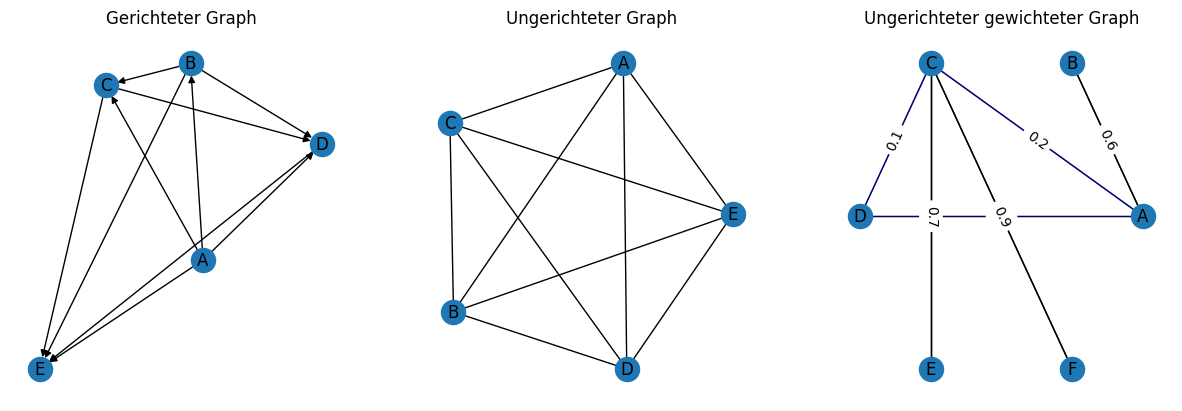
\includegraphics[width=0.9\textwidth]{images/10_introduction/graph_intro.png}
    \caption{Darstellung der verschiedenen Graphen}
    \label{fig:general_graphs}
\end{figure}

Ein Graph kann \textbf{\textit{zusammenhängend}} oder \textbf{\textit{unzusammenhängend}} sein.
Ein zusammenhängender Graph besteht aus einer einzigen zusammenhängenden Komponente, d. h. es gibt einen Pfad von jedem Knoten zu jedem anderen Knoten.
Ein unzusammenhängender Graph besteht aus mehreren Komponenten, die nicht miteinander verbunden sind.

Die \textbf{\textit{Ordnung}} eines Graphen ist die Anzahl der Knoten, die in ihm enthalten sind.
Die Grösse eines Graphen ist die Anzahl der Kanten, die in ihm enthalten sind.
Ein Graph mit $n$ Knoten kann höchstens $\frac{n(n-1)}{2}$ Kanten enthalten, wenn es sich um einen ungerichteten Graphen handelt \cite[p.~48]{barabasi_network_2016}.
Wenn es sich um einen gerichteten Graphen handelt, kann es höchstens $n(n-1)$ Kanten enthalten.

Ein wichtiger Begriff in der Graphentheorie ist der \textbf{\textit{Grad}} eines Knotens, der die Anzahl der Kanten beschreibt, die mit diesem Knoten verbunden sind. Im Falle eines ungerichteten Graphen ist der Grad eines Knotens einfach die Anzahl seiner Nachbarn. Im Falle eines gerichteten Graphen unterscheidet man zwischen dem Eingangsgrad, der Anzahl der Kanten, die auf den Knoten zeigen, und dem Ausgangsgrad, der Anzahl der Kanten, die vom Knoten wegführen. Der Grad eines Knotens kann dazu verwendet werden, die Verbindungsstärke zwischen den Knoten zu beschreiben und somit eine Aussage über die Struktur des Graphen zu treffen \cite[p.~48]{barabasi_network_2016} \cite[p.~14]{harary_graph_1994}.

Eine Möglichkeit, die Verbindungen zwischen den Knoten eines Graphen darzustellen, ist die Verwendung von \textbf{\textit{Adjazenzmatrizen}}. Eine Adjazenzmatrix ist eine quadratische Matrix, die die Verbindungen zwischen den Knoten des Graphen darstellt. Die Einträge der Matrix geben an, ob es eine Verbindung zwischen zwei Knoten gibt oder nicht. Im Falle eines ungerichteten Graphen ist die Adjazenzmatrix symmetrisch. Im Falle eines gerichteten Graphen ist die Adjazenzmatrix nicht symmetrisch. Die Verwendung von Adjazenzmatrizen kann helfen, die Struktur des Graphen zu verstehen und somit Aussagen über seine Eigenschaften und Funktionen zu treffen \cite[p.~51]{barabasi_network_2016} \cite[p.~151]{harary_graph_1994}.

Als Beispiel betrachten wir einen ungerichteten Graphen mit 4 Knoten, der wie folgt dargestellt werden kann:

\[
    A =
    \begin{bmatrix}
        0 & 1 & 1 & 0 \\
        1 & 0 & 1 & 0 \\
        1 & 1 & 0 & 1 \\
        0 & 0 & 1 & 0
    \end{bmatrix}
\]

In diesem Fall ist die Adjazenzmatrix symmetrisch, da der Graph ungerichtet ist. Die Einträge der Matrix geben an, ob es eine Verbindung zwischen zwei Knoten gibt oder nicht. Es gibt so etwa eine Verbindung zwischen Knoten 1 und Knoten 2, da der Eintrag $a_{1,2} = 1$ ist. Es gibt jedoch keine Verbindung zwischen Knoten 1 und Knoten 4, da der Eintrag $a_{1,4} = 0$ ist. Die Verwendung der Adjazenzmatrix kann helfen, die Struktur des Graphen zu visualisieren und Aussagen über seine Eigenschaften zu treffen.

Ein weiterer wichtiger Begriff in der Graphentheorie ist der \textbf{\textit{durchschnittliche Grad}} des Graphen, der angibt, wie viele Kanten jeder Knoten im Durchschnitt hat \cite[p.~48]{barabasi_network_2016}. Für einen ungerichteten Graphen mit $n$ Knoten und $m$ Kanten wird der durchschnittliche Grad $k$ wie folgt definiert:

$$k = \frac{2m}{n}$$

Für gerichtete Graphen unterscheidet man zwischen dem durchschnittlichen Eingangsgrad und dem durchschnittlichen Ausgangsgrad. Der durchschnittliche Grad gibt eine Aussage über die allgemeine Verbindungsstärke im Graphen und kann bei der Identifikation von Clusterstrukturen oder dem Vergleich von Graphen helfen \cite[p.~48]{barabasi_network_2016}.

Ein weiteres wichtiges Konzept in der Graphentheorie ist die \textbf{\textit{Gradverteilung}}. Die Gradverteilung beschreibt, wie viele Knoten in einem Graphen einen bestimmten Grad haben.

$$ P(k) := \frac{\delta_k}{N}$$

Wobei $|V| := N$ und $ \delta_k $ die Anzahl der Knoten mit Grad $k$ ist \cite[p.~311]{emmert-streib_mathematical_2020}.

Eine häufige Gradverteilung ist die Poisson-Verteilung, die für viele zufällige Graphen gilt. Eine andere häufige Gradverteilung ist die Potenzgesetz-Verteilung, die für viele reale Netzwerke gilt, wie in sozialen Netzwerken oder in der Biologie. Die Potenzgesetz-Verteilung ist charakterisiert durch einen hohen Anteil von Knoten mit niedrigem Grad und einem kleinen Anteil von Knoten mit hohem Grad, die als Hubs bezeichnet werden. Die Gradverteilung kann helfen, die Struktur eines Graphen zu verstehen und somit Aussagen über die Funktionsweise des Graphen zu treffen \cite[p.~51]{barabasi_network_2016}.

Die Zentralitätsmasse beschreiben, welche Knoten im Graphen besonders wichtig sind \cite[p.~313]{emmert-streib_mathematical_2020}.
Die Zentralität eines Knotens kann auf verschiedene Arten gemessen werden.
Eine Möglichkeit ist die \textbf{\textit{Degree-Zentralität}}, die angibt, wie viele Kanten mit einem Knoten verbunden sind.
Ein Knoten mit hoher Degree-Zentralität hat viele Nachbarn und ist somit wichtiger als ein Knoten mit niedriger Degree-Zentralität.
Die Degree-Zentralität $C_D(v)$ eines Knotens $v$ in einem ungerichteten Graphen $G=(V,E)$ wird wie folgt definiert:

$$C_D(v) = k_v$$

wobei $k_v$ die Anzahl der Nachbarn von $v$ ist \cite[p.~314]{emmert-streib_mathematical_2020}.

Ein weiteres Mass für die Zentralität ist die \textbf{\textit{Betweenness-Zentralität}}, die angibt, wie oft ein Knoten auf dem kürzesten Pfad zwischen anderen Knoten liegt.
Ein Knoten mit hoher Betweenness-Zentralität spielt eine wichtige Rolle bei der Vermittlung von Information zwischen anderen Knoten.
Die Betweenness-Zentralität $C_B(v)$ eines Knotens $v$ in einem ungerichteten Graphen $G=(V,E)$ wird wie folgt definiert:

$$C_B(v_k) = \sum_{v_i, v_j \in V, v_i \ne v_j} \frac{\sigma_{v_i v_j}(v_k)}{\sigma_{v_i v_j}}$$

wobei $\sigma_{v_i v_j}$ die Anzahl der kürzesten Pfade von $v_i$ nach $v_j$ ist und $\sigma_{v_i v_j}(v_k)$ die Anzahl der kürzesten Pfade von $v_i$ nach $v_j$ durch $v_k$ ist \cite[p.~314]{emmert-streib_mathematical_2020}.


\section{Netzwerkklassen} \label{sec:graph_classes}

Netzwerkklassen sind eine Sammlung von Netzwerken, die bestimmte Eigenschaften teilen.
Diese Eigenschaften können z. B. die Zahl der Knoten, die Anzahl Kanten oder die topologischen Indizes sein.
Brandstädt et al. und später Bang-Jensen et al. sowie Emmert-Streib et al. fassen populäre Graph-Modelle respektive Graphenklassen in verschiedenen Werken zusammen \cite{brandstadt_graph_1999,bang-jensen_basic_2018,emmert-streib_mathematical_2020}.
In den nachfolgenden Abschnitten folgen die bedeutendsten Netzwerkklassen nach \cite{emmert-streib_mathematical_2020}.
Sie bilden die Grundlage für die Weiterarbeit in der Thesis und werden vor allem in der Datenaufbereitung und den Experimenten verwendet.

Nachfolgend werden die Eigenschaften der unterschiedlichen Netzwerkklassen \enquote{Random}, \enquote{Small World} und \enquote{Scale-free} miteinander verglichen.
Dabei werden die Struktur, die Verteilung der existierenden Grade und die Adjazenzmatrix visualisiert und beschrieben.
Zur Einführung sind reguläre, zufällige und Small-World-Graphen auf Abbildung \ref{fig:random_scale_small} visualisiert.

\begin{figure}[H]
    \centering
    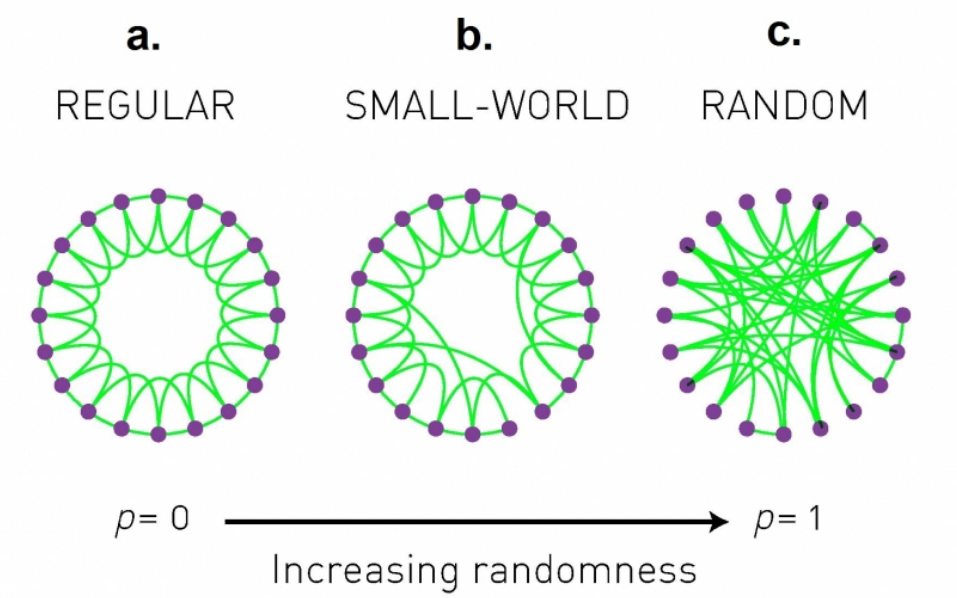
\includegraphics[width=7cm]{images/20_material_methods/barabasi_zusammenhang_smallworld_random.png}
    \caption{Eigenschaften der unterschiedlichen Netzwerkklassen (Quelle: Barabási \cite[p.~97]{barabasi_network_2016})}
    \label{fig:random_scale_small}
\end{figure}

\newpage
\subsection{Random}

Ein Zufallsgraph (engl. random graph) ist ein Graph, der zufällig gemäss einer Wahrscheinlichkeitsverteilung über die Menge aller möglichen Graphen generiert wird.
Das Studium von Zufallsgraphen ist ein Zweig der Graphentheorie und der probabilistischen Kombinatorik.

Ein gängiges Modell zum Erzeugen eines Zufallsgraphen ist das Erdős-Rényi-Modell, bei dem jede mögliche Kante unabhängig mit einer festen Wahrscheinlichkeit $p$ aufgenommen wird \cite[p.~205 ff]{grimmett_random_nodate}.
Dieses Modell ist umfassend untersucht und weist besonders interessante Eigenschaften auf wie den Phasenübergang, der bei der kritischen Wahrscheinlichkeit $p = 1/n$ auftritt, wobei $n$ die Anzahl der Scheitelpunkte im Graphen ist \cite[p.~152]{bollobas_random_2001}.

Des Weiteren ist das bevorzugte Bindungsmodell (engl. preferential attachment) zu nennen, das einen Zufallsgraphen erzeugt, indem es mit einer kleinen Anzahl von Scheitelpunkten beginnt und nacheinander neue Scheitelpunkte hinzufügt, von denen jeder mit einer bestimmten Wahrscheinlichkeit proportional mit vorhandenen Scheitelpunkten verbunden ist \cite[p.~2f]{albert_diameter_1999}.
Dieses Modell wird häufig verwendet, um das Wachstum von sozialen Netzwerken oder des World Wide Web (WWW) zu modellieren.
Es gibt zahlreiche andere Modelle zum Generieren von Zufallsgraphen, jedes hat seine einzigartigen Eigenschaften. Einige Beispiele sind das Small-World, das Watts-Strogatz und das k-reguläre Modell \cite[p.~398f.]{newman_networks_2010}.

Das Studium von Zufallsgraphen hat zu einem tieferen Verständnis der Struktur und Eigenschaften realer Graphen sowie zur Entwicklung effizienter Algorithmen zum Generieren und Analysieren grosser Graphen geführt.
Auf Abbildung \ref{fig:random_graphs} sind drei Zufallsgraphen ersichtlich; gewisse Knoten besitzen einen Grad $k = 0$, was bedeutet, dass sie isoliert sind und keine Kanten haben \cite[p.~85]{barabasi_network_2016}:

\begin{figure}[H]
    \centering
    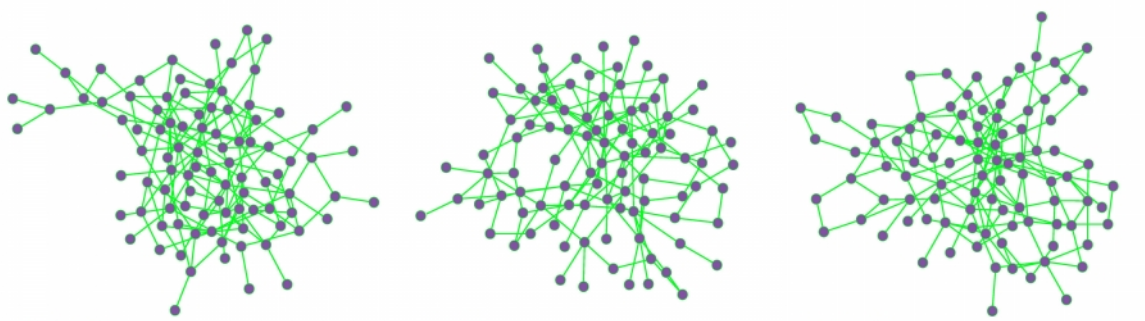
\includegraphics[width=11cm]{images/20_material_methods/random_graphs.png}
    \caption{Drei Random-Graphen mit $\protect p = 0.03$ und $\protect N = 100 $ (Quelle: Barabási. \cite[p.~84]{barabasi_network_2016})}
    \label{fig:random_graphs}
\end{figure}

\newpage
\subsection{Small World}

Ein Small-World-Graph ist eine Art komplexes Netzwerk, das sowohl eine hohe Clusterbildung als auch eine kurze durchschnittliche Pfadlänge aufweist.
Das Konzept der Small-World-Graphen ist erstmals in den 1960er-Jahren von Stanley Milgram durch das \enquote{Six Degrees of Separation}-Experiment eingeführt worden.
Er hat gezeigt, dass zwei beliebige Menschen auf der Erde durchschnittlich über sechs Bekanntschaften verbunden sind  \cite[p.~62]{travers_experimental_1969}

Ende der 1990er-Jahre haben Duncan J. Watts und Steven H. Strogatz das Konzept der Small-World-Graphen weiterentwickelt und den Begriff \enquote{Small-World Networks} eingeführt \cite[p.~440]{watts_collective_1998}.
Sie haben damit gezeigt, dass Small-World-Netzwerke durch eine hohe Clusterbildung gekennzeichnet sind, was bedeutet, dass Knoten in der Regel mit anderen Knoten zusammenhängen, die wiederum eng mit diesen verbunden sind, genauer gesagt durch eine kurze durchschnittliche Pfadlänge.
Dies heisst, dass es unkompliziert ist, jeden Knoten im Netzwerk durch eine vergleichsweise kleine Anzahl von Schritten zu erreichen.

Watts und Strogatz (1998) definieren in ihrem Modell zum Aufbau von Small-World Networks $n$ Knoten, wobei jeder Knoten mit $m$ nächsten Nachbarn verbunden ist.
Dies wird als reguläres Gitter bezeichnet (siehe Abbildung \ref{fig:small_world}), wobei $n = 10$ und $m = 4$ ist  \cite{gayen_small_2020}.
\begin{figure}[H]
    \centering
    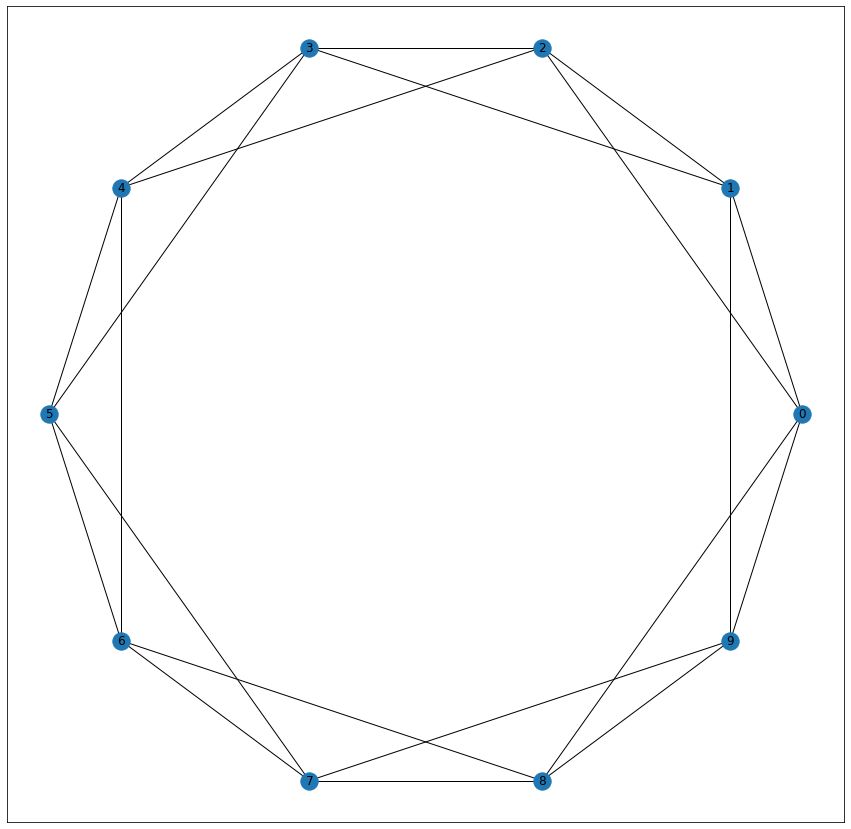
\includegraphics[width=3cm]{images/20_material_methods/small_world_lattice.png}
    \caption{Regular Lattice Graph (Quelle: Gayen \cite{gayen_small_2020})}
    \label{fig:small_world}
\end{figure}
Bei Betrachtung einer jeden Kante $(u, v)$ wird mit der Wahrscheinlichkeit $p$ zufällig ein Knoten $w$ ausgewählt und die Kante $(u, v)$ so verbunden, dass sie zu $(u, w)$ wird.
Für $p = 0$ behält es seine Struktur und hat einen hohen durchschnittlichen Abstand und eine hohe Clusterbildung.
Für $p = 1$ wird ein Zufallsnetzwerk mit kleiner durchschnittlicher Distanz und geringer Clusterbildung gebildet \ref{fig:small_world_lattice_n10}, wobei $n = 10$, $m = 4$ und $p = 1$ ist.
Für einen Zwischenwert von $p$ erhält man ein ideales Small-World Network mit geringer durchschnittlicher Entfernung und hoher Clusterbildung \cite{gayen_small_2020}.
\begin{figure}[H]
    \centering
    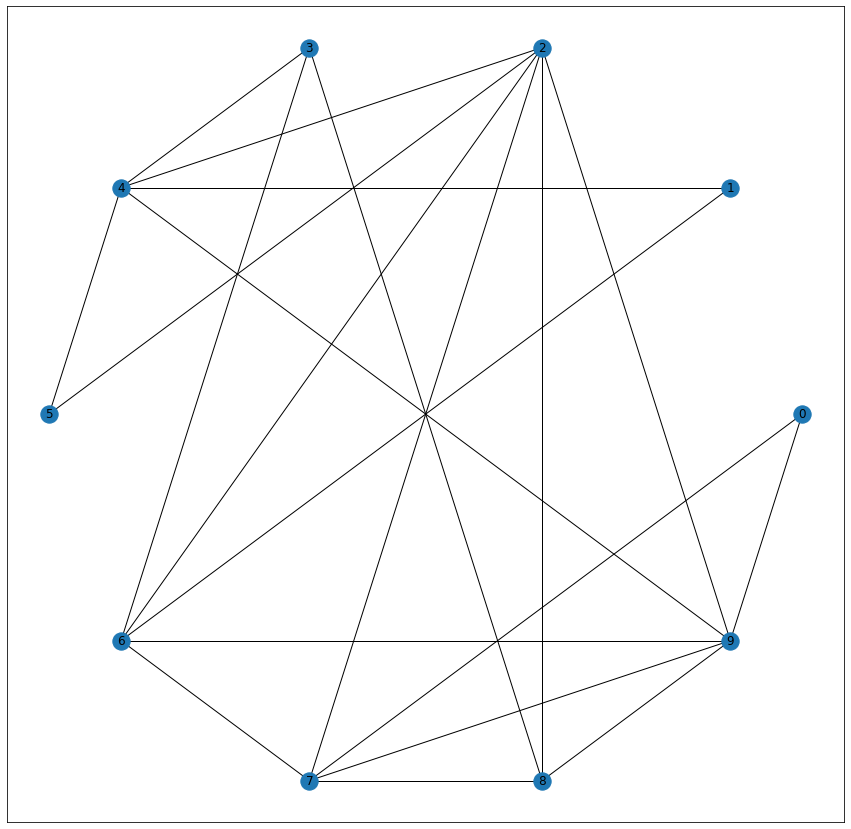
\includegraphics[width=3cm]{images/20_material_methods/small_world_lattice_n10.png}
    \caption{Regular Lattice Graph mit $n = 10, m = 4$ und $p = 1 $ (Quelle: Gayen \cite{gayen_small_2020})}
    \label{fig:small_world_lattice_n10}
\end{figure}
Es hat sich herausgestellt, dass Small-World-Graphen in Systemen der realen Welt weitverbreitet sind, darunter soziale Netzwerke, Transportnetzwerke und das Internet \cite[p.~4]{barabasi_emergence_1999}.
Sie werden auch in verschiedenen Bereichen wie Physik, Biologie und Informatik untersucht, da sie bedeutende Auswirkungen auf die Verbreitung von Informationen und die Robustheit von Netzwerken haben \cite[p.~2]{newman_structure_2003}.

\subsection{Scale-free}

In der Anfangsphase des Web, in den 1990er-Jahren, wurde davon ausgegangen, dass dieses die Eigenschaften eines zufälligen Netzwerks hat, des Netzwerktyps, der von Erdős–Rényi (1960) mathematisch charakterisiert wurde und in dem die Wahrscheinlichkeit für die Verbindung zweier Knoten als Konstante angegeben ist.
In einem derartigen Netzwerk folgt die Gradverteilung der Poisson-Form \cite{barabasi_network_2016}.

Albert et al. (1999, S. 1) haben gezeigt, dass das WWW nicht diese zufällige Netzwerkstruktur hat \cite{albert_diameter_1999}.
Tatsächlich ist die Gradverteilung ein Potenzgesetz, bei dem die Wahrscheinlichkeit, dass ein Knoten den Grad $k$ hat, proportional zu $k-\lambda$ ist, wobei $\lambda$ etwa $2$ ist.
Ein solches Netzwerk hat andere Eigenschaften, als ein zufälliges Netzwerk, da ein Potenzgesetz weniger stark abfällt als eine Poisson-Kurve.
Anstatt dass praktisch alle Knoten mehr oder weniger den gleichen Grad haben, sind einige wenige Knoten äusserst stark verbunden und die überwiegende Mehrheit hat einen geringeren Grad als der Durchschnitt \cite{barabasi_network_2016}.

\subsection{Bäume}

Ein Baum (engl. Tree) ist ein gerichteter Graph, der keine Schleifen und Kreise enthält.
Das bedeutet, dass jeder Knoten genau einen Vorgänger hat und dass es einen eindeutigen Pfad von jedem Knoten zum Wurzelknoten gibt \cite{cayley_analytical_1881}.

Die Verwendung von Bäumen ist eine gängige Methode zur Simulation von Hierarchien und Untersuchung von Struktureigenschaften in komplexen Netzwerken.
Zum Beispiel kann ein Baum Graph verwendet werden, um die Verteilung von Informationsflüssen in einem Netzwerk zu untersuchen oder um die Effekte von Strukturänderungen auf die Effizienz von Netzwerken zu bewerten \cite{brandstadt_graph_1999}.

Ein weiterer Vorteil von Baum Graphen ist, dass sie einfach zu generieren sind und wenig Rechenaufwand erfordern.
Daher sind sie für Anwendungen zweckmässig, bei denen schnelle und einfache Simulationen erforderlich sind, insbesondere bei der Analyse von grossen Netzwerken. Zudem können Baum Graphen auch verwendet werden, um statistische Eigenschaften komplexer Netzwerke zu schätzen, etwa die Verteilung von Knotengrössen oder die Anzahl der Verbindungen zwischen Knoten.

Insgesamt bieten Baum Graphen eine geeignete Methode zur Analyse von Hierarchien und Strukturen in komplexen Netzwerken.
Sie benötigen wenig Rechenaufwand und bieten relevante Informationen über die Eigenschaften von Netzwerken.
Daher sind sie ein wesentlicher Bestandteil der Netzwerktheorie und werden oft in der Praxis verwendet \cite{cayley_analytical_1881,emmert-streib_mathematical_2020}.

\begin{figure}[H]
    \centering
    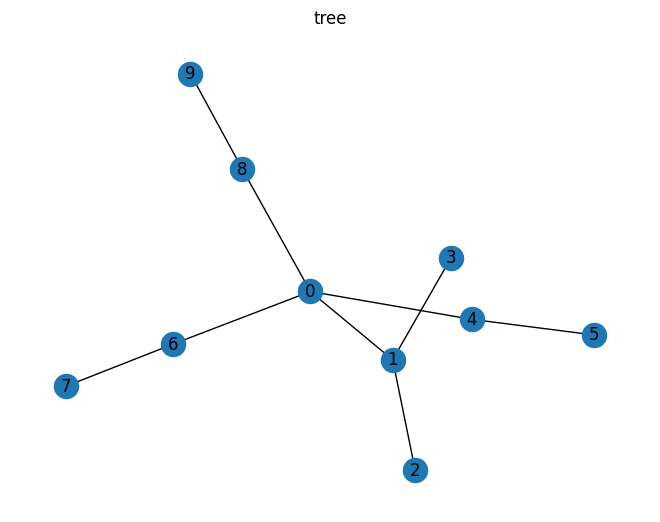
\includegraphics[width=6cm]{images/20_material_methods/tree.png}
    \caption{Baum Graph}
    \label{fig:tree-graph}
\end{figure}

\subsubsection{Sterne}

Sterngraphen sind eine Klasse von ungerichteten Graphen und eine Unterklasse von Bäumen, bei denen ein Knoten (zentraler Knoten) direkt mit allen anderen Knoten (Peripherie-Knoten) verbunden ist. 
Ein Sterngraph mit $n$ Knoten kann als $S_n$ dargestellt werden. 
Der zentrale Knoten in einem Sterngraphen hat $n-1$ Kanten, während jeder Peripherie-Knoten nur eine Kante hat.

Die Formel für die Anzahl der Kanten eines Sterngraphen lautet:
\begin{equation}
    \text{E}(S_n) = n-1
\end{equation}
Sterngraphen haben folgende Eigenschaften:
\begin{enumerate}
    \item Sie besitzen $n$ Knoten und $n-1$ Kanten.
    \item Sie haben keine Schleifen.
    \item Ihr Durchmesser ist $\min{2, n}$.
    \item Sie sind zusammenhängend.
\end{enumerate}

Sie sind einfach zu konstruieren und zu analysieren und werden oft verwendet, um Probleme in verschiedenen Bereichen zu lösen.

\begin{figure}[H]
    \centering
    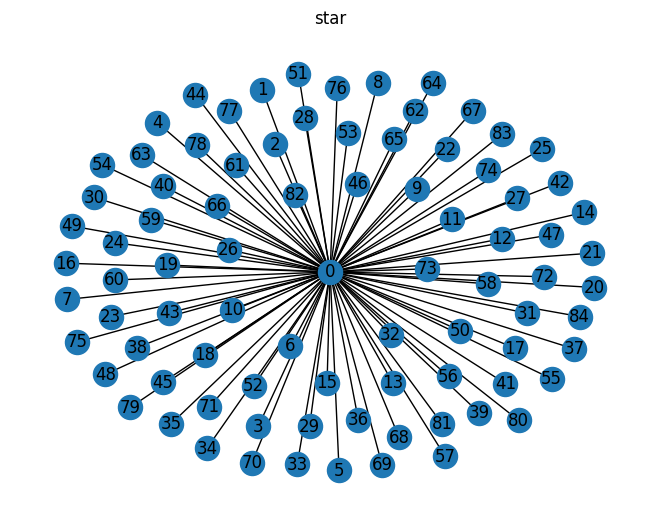
\includegraphics[width=6cm]{images/20_material_methods/star.png}
    \caption{Sterngraph}
    \label{fig:star-graph}
\end{figure}

\subsection{Vollständig} \label{sec:complete}

Vollständige Graphen sind eine bedeutsame Klasse von Graphen in der Mathematik, die eine vollständige Verbindung aller Knoten innerhalb des Graphen darstellen.
Bei einem vollständigen Graphen mit $n$ Knoten ist jeder Knoten mit jedem anderen direkt verbunden.
Ein vollständiger Graph mit $n$ Knoten kann als $G(n)$ dargestellt werden.

Die Formel für die Anzahl der Kanten eines vollständigen Graphen lautet \cite[p.~53]{barabasi_network_2016}:
\begin{equation}
    \text{E}(G(n)) = \frac{n(n-1)}{2}
\end{equation}

Ein Complete Graph ist ein besonderer Fall des k-regulären Graphen, bei dem jeder Knoten eine gleichmässige Anzahl von Kanten hat.
Er ist der maximale k-reguläre Graph für $k = n-1$ \cite{bang-jensen_basic_2018}.

\begin{figure}[H]
    \centering
    \includesvg[width=4cm]{images/20_material_methods/k5-graph.svg}
    \caption{K5-Graph}
    \label{fig:k5-graph}
\end{figure}

\subsection{Path}

Path Graphs, auch bekannt als Pfadgraphen, sind eine einfache Klasse von Graphen, die eine gerichtete Kette von Knoten darstellen.
Ein Path Graph mit $n$ Knoten kann als $P_n$ dargestellt werden.
Jeder Knoten in einem Pfadgraphen hat genau eine eingehende und eine ausgehende Kante, ausser dem ersten Knoten, der nur eine ausgehende, und dem letzten Knoten, der nur eine eingehende Kante hat.

Die Formel für die Anzahl der Kanten eines Path Graph lautet:
\begin{equation}
    \text{E}(P_n) = n-1
\end{equation}

Path Graphs finden häufig Anwendung in der Mathematik, insbesondere bei der Untersuchung von Problemen in der Graphtheorie und Netzwerktheorie \cite{bender_lists_2010}. 
Zum Beispiel können Path Graphs verwendet werden, um den kürzesten Pfad in einem Netzwerk zu untersuchen, und sie können auch als Bausteine für die Konstruktion von grösseren Graphen verwendet werden.

\begin{figure}[H]
    \centering
    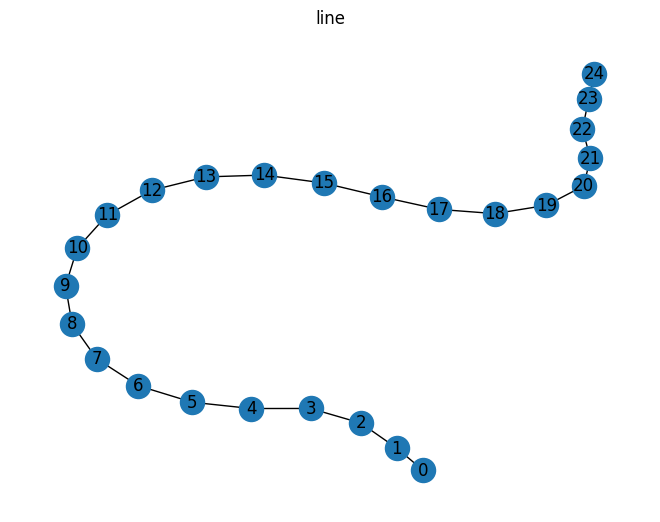
\includegraphics[width=6cm]{images/20_material_methods/path.png}
    \caption{Path oder Line Graph}
    \label{fig:path-graph}
\end{figure}


\newpage
\section{Topologische Indizes} \label{sec:topologische_indizes}

Topologische Indizes sind mathematische Masse, die die topologische Struktur eines Graphen charakterisieren.
Sie können genutzt werden, um die Konnektivität oder Komplexität eines Netzwerks zu beschreiben, und sie haben zahlreiche Anwendungen in einer Vielzahl von Bereichen:
In der Chemie dienen topologische Indizes dazu, die Eigenschaften chemischer Verbindungen wie Siede-, Schmelzpunkte und Löslichkeit vorherzusagen.
Sie können auch verwendet werden, um die strukturellen und funktionellen Eigenschaften von Biomolekülen wie Proteinen und Nukleinsäuren zu untersuchen.
In der Biologie kann mithilfe von topologischen Indizes, um die Protein-Ligand-Bindungsaffinität vorhergesagt werden, was für das Arzneimitteldesign bedeutsam ist.
Topologische Indizes können auch zur Untersuchung der Struktur und Funktion biologischer Netzwerke eingesetzt werden, etwa Protein-Protein-Interaktionsnetzwerke und metabolische Netzwerke \cite[p.~199ff]{balaban_topological_1983}.
In sozialen Netzwerken können topologische Indizes verwendet werden, um die Struktur von Netzwerken zu analysieren und zu verstehen, wie sich Informationen durch diese verbreiten.

Der topologische Index ist ein numerischer Wert oder eine Sequenz für eine bestimmte diskutierte Struktur, die tatsächlich die physikalischen, chemischen und biologischen Eigenschaften eines Graphen abbildet \cite{manzoor_entropy_2020}.
Einige Indizes spiegeln die Grösse des Moleküls wider, z. B. der Kohlenstoffzahlindex, andere, z. B. der Balaban-Zentralindex, charakterisieren die Form \cite[p.~1]{rouvray_modeling_1987}.
\begin{theorem}[Topologischer Index]
    \label{thm:topologischer_index}%
    Ein topologischer Index ist eine numerische Invariante eines Graphen \cite[p.~235]{plavsic_harary_1993}.

    Topologische Indizes sind Zahlen, welche Graphen durch konstitutionelle Formeln aus mathematischen Operationen als numerische Werte repräsentieren. \cite[p.~16]{devillers_topological_2000}, \cite[p.~23]{devillers_topological_2000}.
\end{theorem}

\newpage
\subsection{Anwendung von topologischen Indizes}

Eine der Hauptanwendungen topologischer Indizes ist die Untersuchung der Eigenschaften chemischer Verbindungen, um diese basierend auf ihren strukturellen und funktionellen Eigenschaften zu klassifizieren. Topologische Indizes werden auch zugrunde gelegt, um die Struktur und Funktion von Biomolekülen wie Proteinen und Nukleinsäuren zu untersuchen \cite[p.~1015]{gonzalez-diaz_medicinal_2007}.
Topologische Indizes dienen auch dazu, wesentliche Einflussfaktoren zu identifizieren oder vorherzusagen, wie sich das Netzwerk im Laufe der Zeit verändern könnte \cite[p.~400]{watts_collective_1998}.

Topologische Indizes werden auch angewendet, um Probleme in anderen Bereichen wie Informatik, Ingenieurwesen und Wirtschaftswissenschaften zu lösen. So werden sie beispielsweise eingesetzt, um den kürzesten Weg zwischen zwei Punkten in einem Transportnetzwerk zu finden \cite{dijkstra_note_1959} und um die Ressourcenallokation in einer Lieferkette zu optimieren \cite{bazaraa_nonlinear_2013}.
Insgesamt liegt der Nutzen topologischer Indizes in ihrer Fähigkeit, ein quantitatives Mass für die topologische Struktur eines Graphen bereitzustellen, das zur Untersuchung der Eigenschaften komplexer Systeme und zur Lösung von Problemen in einer Vielzahl von Bereichen verwendet werden kann.

Topologische Indizes werden u. a. von Chemikern als Werkzeug zur Beschreibung chemischer Phänomene genutzt.
Die topologischen Indizes charakterisieren dabei sowohl die Grösse als auch die Form chemischer Spezies und spiegeln die Menge an Verzweigungen in Molekülen signifikant wider.
Chemiker sind somit in der Lage, das chemische Verhalten einer breiten Palette chemischer Substanzen in allen drei thermodynamischen Zuständen graphenbasiert genau zu modellieren \cite[p.~1]{rouvray_modeling_1987}.

Eine ihrer Eigenschaften, die als Einzigartigkeit oder Unterscheidungskraft bezeichnet wird, ist in der mathematischen Chemie und im strukturorientierten Arzneimitteldesign im Kontext der quantitativen Charakterisierung der Struktur von Molekülen ausführlich untersucht worden.
Im Allgemeinen erhält ein Index das Attribut degeneriert, wenn er für mehr als einen Graphen denselben Wert besitzt \cite[p.~1]{dehmer_information_2012}.

Weitere Wissenschaftler haben magnitudenbasierte Informationsindizes vorgeschlagen, um die Trennschärfe anderer klassischer topologischer Index für Alkanbäume und Isomere zu verbessern.
Alkanbäume sind zusammenhängende und azyklische Graphen, in denen der Grad eines Knotens höchstens 4 ist.
Zudem wird die Trennschärfe von informationstheoretischen Massen basierend auf Distanzen für chemische Graphen unterschieden, die einen Ring enthalten.
So ist die Einzigartigkeit verschiedener informationstheoretischer und nicht informationstheoretischer Massnahmen gegeben, indem polyzyklische Strukturen verwendet werden.
Als Ergebnis erweisen sich der Balaban-J-Index, die Summe der lokalen Vertex-Entropien und die magnitudenbasierten Informationsindizes als einzigartig, für diese Klasse von Graphen \cite[p.~1]{dehmer_information_2012}.

Neben empirischen Eigenschaften von Informationsmassen für Graphen – etwa das Bestimmen von Korrelationen zwischen den Massen – bestehen auch mathematische Probleme, z. B. der Nachweis verschiedener Ober- und Untergrenzen von Massnahmen.
Die Korrelationsfähigkeit zwischen zwei Graphmassen bezieht sich im Allgemeinen auf das Problem, ob sie strukturelle Informationen ähnlich erfassen.
Ausserdem wird die Klasse der Graphen-Entropiemasse, die durch Verwendung bestimmter Informationsfunktionale auf Grundlage der metrischen Eigenschaften von Graphen (z. B. der Nachbarschaft von Atomen) erhalten werden, verwendet, um Probleme in QSAR und QSPR zu lösen.
Insbesondere Dehmer et al. (2012) klassifizieren die sog. Mutagenität von Molekülen unter Verwendung dieser Massnahmen und unter Nutzung überwachter Lerntechniken \cite[p.~2]{dehmer_information_2012}.

Insgesamt werden in dieser Studie die Grenzen topologischer Indizes und Restriktionen bei deren Anwendung im grossen Massstab deutlich. Ein topologischer Index kann für eine bestimmte Graphenklasse eindeutig sein, aber er schlägt fehl, wenn das Mass auf eine andere Klasse angewendet wird \cite[p.~9]{dehmer_information_2012}.

Topologische Indizes \(TI(G)\) haben folgenden Anforderungen zu erfüllen:

\begin{lemma}[Topologische Indizes und Isomorphie]
    \label{thm:index_isomorphism}%
    Wenn \(G_1 \simeq G_2 \) (isomorph) sind, dann gilt \(TI(G_1) = TI(G_2)\).
    Im Umkehrschluss gilt bei \(TI(G_1) = TI(G_2)\), \( G_1 \simeq G_2\) nicht, da Indizes bei nicht isomorphen Graphen auch denselben Wert ergeben können.
\end{lemma}

Dieses Lemma wird in den zwei nachstehenden Beispielen verdeutlicht.

\begin{figure}[H]
    \begin{subfigure}{.4\textwidth}
        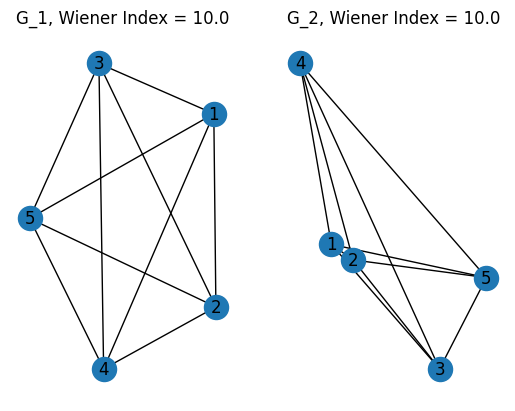
\includegraphics[width=\textwidth]{images/20_material_methods/lemma_2_proof_1.png}
        \label{fig:lemma_proof_1}
    \end{subfigure}%
    \hfill
    \vline
    \hfill
    \begin{subfigure}{.4\textwidth}
        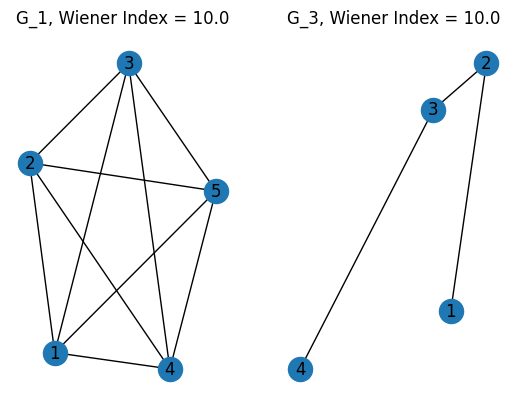
\includegraphics[width=\textwidth]{images/20_material_methods/lemma_2_proof_2.png}
        \label{fig:lemma_proof_2}
    \end{subfigure}
    \caption{Nachweis von Lemma \ref{thm:index_isomorphism}. G\_1 und G\_2 links, sind isomorphe Graphen. G\_1 und G\_3 in der rechten Abbildung sind nicht isomorphe Graphen, aber haben denselben Wiener Index.}
\end{figure}

Die topologischen Indizes können nach Balaban in verschiedene Kategorien eingeteilt werden \cite{balaban_1983_2014}.
Dabei spricht er von den folgenden Klassen: gradbasiert (Adjazenzmatrix), distanzbasiert (Distanz-Matrix), zentrische Indizes und informationstheoriebasiert.

\subsection{Gradbasiert}

Sei $\mathcal{G}$ ein molekularer Graph. Zwei Knoten von $\mathcal{G}$, die durch eine Kante verbunden sind, heissen \enquote{benachbart}.
Sind zwei Knoten $u$ und $v$ benachbart, besteht die Beziehung $u ~ v$.
Die Anzahl der Knoten von $\mathcal{G}$, die an einen gegebenen Knoten $v$ angrenzen, ist der \enquote{Grad} dieses Knotens und wird mit $dv(\mathcal{G})$ bezeichnet – wenn die Eindeutigkeit gegeben ist, mit $dv$.
Das Konzept des Grades in der Graphentheorie ist eng verwandt mit dem Konzept der Valenz in der Chemie \cite[p.~351]{gutman_degree-based_2013}.

\begin{figure}[H]
    \centering
    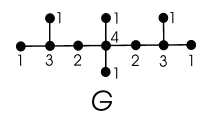
\includegraphics[width=0.3\textwidth]{images/20_material_methods/degree_graph.png}
    \caption{Graph $\mathcal{G}$ mit den Knotengeraden (Quelle: \cite[p.~351]{gutman_degree-based_2013})}
    \label{fig:degree_graph}
\end{figure}

Somit hat $\mathcal{G}$ sechs Knoten vom Grad $1$ (sogenannte \enquote{hängende} Knoten, die Methylgruppen darstellen) und zwei Knoten vom Grad 2 sowie zwei vom Grad 3 und einen Knoten vom Grad 4. Aus chemischen Gründen können die molekularen Graphen von Kohlenwasserstoffen keine Knoten besitzen, deren Grad grösser als 4 ist \cite[p.~351]{gutman_degree-based_2013}.

\subsubsection{Randić-Index}

Der Randić-Index und der Generalized Randić-Index sind Masse für die Struktur von Molekülen in der Chemie.
Der Randić-Index wurde von Milan Randić entwickelt und ist ein Mass für die \enquote{Heterogenität} oder die Unterschiedlichkeit der Atome in einem Molekül \cite{li_survey_2008}.

Er wird wie folgt berechnet:
\begin{equation}
    R = \sum_{uv \in E(G)}\frac{1}{\sqrt{d_u d_v}}
\end{equation}
Hierbei ist $d(i)$ die Anzahl der Nachbarn des Atoms $i$ und die Summe läuft über alle Atome des Moleküls.

Im Jahr 1998 haben Bollobás und Erdős den generalized Randić Index definiert, bei welchem auch die Anzahl der Bindungen zwischen den Atomen berücksichtigt wird \cite{li_survey_2008}.

Er wird folgendermassen berechnet:
\begin{equation}
    R_{\alpha}(G) = \sum_{uv \in E}{d(u) d(v)}^{\alpha}
\end{equation}
Im Allgemeinen wird der Generalized Randić-Index verwendet, wenn mehr Informationen über die Struktur eines Moleküls erlangt werden sollen, insbesondere über die Anzahl und Art der Bindungen zwischen den Atomen.
Der Randić Index hingegen ermöglicht nur Informationen über die Anzahl der Nachbarn eines Atoms und ist daher weniger detailliert.

Des Weiteren ist der $R_{\alpha}$ mit einem $\alpha = +1$ unter dem Namen \textit{Second Zagreb Index} definiert \cite{li_survey_2008}.

\subsubsection{Zagreb-Index}

Der erste Zagreb-Index wurde 1972 von Gutman und Trinajstic definiert \cite{xu_zagreb_2011}.
Er ist gleich der Summe der quadrierten Nachbarschaftsgrade aller Knoten.
\begin{equation}
    M_1(G) = \sum_{u \in V (G)} deg(v)^2
\end{equation}
Der zweite Zagreb-Index wird folgendermassen definiert:
\begin{equation}
    M_2(G) = \sum_{uv \in E (G)} deg(u) deg(v)
\end{equation}
Er ist die Summe der Produkte der Knotengrade von benachbarten Knoten \cite{das_zagreb_2015}.

\subsubsection{Harmonischer Index}

Der harmonische Index ist eine Variante des Randić-Index \cite[p.~562]{zhong_harmonic_2012}.
Er ist als die Summe der Gewichte aller Kanten von $uv$ von $G$ definiert, wobei $d(u)$ den Grad eines Knotens $u$ in $G$ abbildet.
Für einen Graphen $G$ lautet wird er wie berechnet \cite[p.~562]{zhong_harmonic_2012}:
\begin{equation}
    H(G) = \sum_{uv \in E (G)} \frac{2}{d(u) + d(v)}
\end{equation}
Die Berechnung des harmonischen Index kann aufwendig sein, insbesondere für grosse Graphen, aber es gibt Algorithmen und Techniken, um ihn effizient zu berechnen. 
Der harmonische Index hat auch interessante mathematische Eigenschaften und ist ein aktives Forschungsgebiet in der Graphentheorie \cite{li_harmonic_2014}.

\subsubsection{Atom-Bond Connectivity Index}

Dieser Index beschreibt die Verbindungen zwischen den Atomen einer Verbindung und berechnet den Index auf der Basis der Anzahl der Bindungen, die jedes Atom hat.
Die Verwendung von gradbasierten Metriken zur Charakterisierung von Verbindungen ist ein bedeutender Aspekt in der chemischen Informatik, und der Atom-Bond-Connectivity (ABC) Index ist eine gängige Methode zur Bewertung der Atomkonnektivität in Verbindungen \cite{estrada_atom-bond_1998}.

Die Formel zur Berechnung des ABC-Index lautet:
\begin{equation}
    ABC = \sum_{uv \in E(G)} \sqrt{\frac{d_u + d_v - 2} {d_u \times d_v}}
\end{equation}
Hierbei sind $d_u$ und $d_v$ die Grade der Knoten $u$ und $v$.

\subsection{Distanzbasiert}

\subsubsection{Wiener-Index}

Der Wiener-Index ist der erste topologische Index, der von Harold Wiener, einem Chemiker, eingeführt wurde \cite{fath-tabar_hyper-wiener_2011}.
Ein fundamentaler, distanzbasierter Index ist der Wiener-Index. Er ist als Summe der Abstände zwischen allen ungeordneten Scheitelpunktpaaren des Graphen definiert und heute aufgrund des breiten Anwendungsspektrums weitgehend verbreitet.
Insbesondere ist er einer der am häufigsten verwendeten topologischen Indizes in der mathematischen Chemie.
Angesichts dessen korreliert es stark mit vielen physikalischen und chemischen Eigenschaften molekularer Verbindungen, deren Eigenschaften nicht nur von ihrer chemischen Formel, sondern auch von ihrer molekularen Struktur abhängen \cite[p.~2]{cavaleri_group_2021}.
Es werden die Summen aller Abstände (kürzeste Wege) von jedem Knoten zu jedem anderen Knoten in die Berechnung einbezogen.
Der Wiener-Index ist definiert durch \cite[p.~17]{wiener_structural_1947}:
\begin{equation}
    W = \frac{1}{2}\sum^N_{i,j}d_{ij}
\end{equation}

\subsubsection{Hosoya-Index} \label{sec:hosoya_index}

Der Hosoya-Index, auch molekularer topologischer Index genannt, ist ein mathematisches Mass für die topologische Komplexität eines Moleküls.
Er ist definiert als die Summe der Quadrate des Grades jedes Scheitelpunkts im Molekulargraphen, wobei der Grad eines Scheitelpunkts die Anzahl der damit verbundenen Kanten ist.
Der Hosoya-Index korreliert nachweislich mit verschiedenen physikalischen und chemischen Eigenschaften von Molekülen wie Siedepunkt und Löslichkeit \cite[p.~397ff]{hosoya_topological_1972}.

Eine der frühesten wissenschaftlichen Arbeiten zum Hosoya-Index ist 1981 von F. Hosoya und Y. Tanaka in der Zeitschrift Chemical Physics Letters veröffentlicht worden.
In diesem Artikel stellen die Autoren das Konzept des Hosoya-Index vor und demonstrieren sein Potenzial als Mass für die molekulare Komplexität.
Seit seiner Einführung ist der Hosoya-Index auf dem Gebiet der chemischen und biochemischen Forschung weitverbreitet und Gegenstand zahlreicher wissenschaftlicher Arbeiten und Übersichtsartikel \cite[p.~397ff]{hosoya_topological_1972}.

Er wird folgendermassen berechnet \cite[p.~182]{hosoya_topological_1972}:
\begin{equation}
    Z = \sum_{k = 0}^{\lfloor N / 2 \rfloor} p(G, k)
\end{equation}
Dabei ist $ p(G, k) $ die Anzahl Möglichkeiten, in welcher $ k $ Knoten von $ G $ gewählt werden können, so dass keine zwei Knoten benachbart sind.
Das in den Gauss-Klammern stehende $ N / 2 $ ist die kleinste natürliche Zahl innerhalb $ N / 2 $.
Den grössten Hosoya-Index eines Graphen mit $ n $ Knoten erhält man von einem kompletten Graphen \ref{sec:complete}.

\subsubsection{Szeged-Index}

Der Szeged-Index ist ein Mass für den Informationsgehalt eines Graphen und wird verwendet, um die Komplexität oder Struktur des Graphen zu bewerten.
Er ist von Ivàn Gutman 1994 eingeführt worden und generalisiert das Konzept des Wiener-Index \cite{gutman_szeged_1998}.

Er lässt sich folgendermassen berechnen \cite[p.~2]{gutman_szeged_1998}:
\begin{equation}
    Sz(G) = \sum_{e \in E(G)} n_1(e | G)n_2 (e | G)
\end{equation}
Hier ist $ e $ eine Kante aus $ E $ im Graphen $ G $; $ e $ verbindet die Knoten $ u $ und $ v $, so wird auch $ e = uv $ oder $ e = vu $ geschrieben.
Für $ e = uv \in E(G) $ sei $ n_1(e | G) $ und $ n_2(e | G) $ die Anzahl Knoten von $G$, die näher zu Knoten $ u $ als Knoten $ v $ respektive für $n_2$ näher bei Knoten $ u $ als Knoten $ v $ sind \cite{gutman_szeged_1998}.

\subsection{Zentrische Indizes}

Die zentrischen Indizes wurden durch Balaban eingeführt und sind eine Gruppe von Indizes, die die zentrische Struktur eines Graphen beschreiben \cite{balaban_1983_2014}.
Sie verhalten sich ähnlich wie die Distanz-Indizes, da es bei der Suche nach dem zentralen Knoten auf die Distanz zwischen den Knoten ankommt.
Gemäss dem Jordanschen Zentrumssatzes ist der zentrische Knoten derjenige, der die geringste Summe der Distanzen zu allen anderen Knoten hat \cite[p.~32]{gross_graph_2018}. \\
Die Definition des Zentrums eines Graphens $ G $ ist eine Menge von Knoten $ V $, deren \textit{graph eccentricity} gleich dem Graph-Radius ist \cite[p.~35]{harary_graph_1994}.

\subsubsection{Balabans zentrischer Index B}

Der zentrische Index $B$ von Balaban wurde Entwickelt, um das Zentrum von Baumgraphen zu bestimmen \cite[p.~355]{balaban_chemical_1979}.
$ B $ wird ähnlich wie der erste Zagreb-Index aufgrund der quadratischen Formel definiert \cite[p.~355]{balaban_chemical_1979}.
\begin{equation}
    B = \sum_{i} \delta_i^2
\end{equation}

Dabei ist $ \delta_i $ die Anzahl Knoten, welche bei jedem Schritt $ i $ entfernt werden können, ohne dass der Graph zerfällt \cite[p.~355]{balaban_chemical_1979}.

\subsubsection{Estrada-Index}

Der Estrada-Index $ EE $ ist ein topologischer Index, welchen Estrada im Jahr 2005 eingeführt hat \cite{estrada_subgraph_2005}. 
Seinen Namen hat er jedoch erst 2007 von de la Peña \cite{de_la_pena_estimating_2007} erhalten. Er misst die Partizipation von allen Knoten in allen Teilgraphen eines Graphen \cite[p.~6]{estrada_subgraph_2005} und wird wie folgt berechnet \cite[p.~6]{estrada_subgraph_2005}:
\begin{equation}
    EE(G) = \sum_{i=1}^n e^{\lambda_i}
\end{equation}
Es ist $ G $ der Graph, $ n $ die Anzahl der Knoten und $ \lambda_i $ sind die Eigenwerte der Adjazenzmatrix $ A $.

\subsection{Informationstheoriebasiert}

Unter \enquote{Informationstheorie} wird ein Zweig der Mathematik verstanden, in dem die Quantifizierung und Analyse von Informationen thematisiert wird \cite[p.~82-83]{dehmer_information_2008}.
Informationstheoriebasierte Indizes stellen Masse dar, die Prinzipien der Informationstheorie verwenden, um den Informationsgehalt oder die Komplexität eines Systems quantitativ zu bewerten.
Ein Beispiel für einen auf der Informationstheorie basierenden Index ist die Entropie, die ein Mass für das Ausmass der Unsicherheit oder Zufälligkeit in einem System darstellt \cite[p.~767-768]{dehmer_information_2011}.
Entropie kann verwendet werden, um den Informationsgehalt einer Nachricht zu messen, indem bspw. das Ausmass der Unsicherheit quantifiziert und durch Erhalt der Nachricht reduziert wird \cite[p.~3]{iceland_multigroup_2004}.
Newman \cite[p.~2ff]{newman_structure_2003} diskutiert in diesem Kontext die Verwendung informationstheoretischer Indizes, einschliesslich der Entropie und gegenseitiger Informationen, um die Entwicklung von Informationen in komplexen Systemen zu untersuchen, die Zentralität von Knoten in Netzwerken zu quantifizieren sowie die Struktur und Funktion komplexer Netzwerke zu analysieren.

Balaban \cite[p.~16]{balaban_1983_2014} beschreibt zudem, dass laut einer Untersuchung die diversen informationstheoretischen Indizes eine tiefe diskriminierende Leistung aufweisen, was bedeutet, dass sie in der Lage sind, die Struktur eines Graphen zu unterscheiden, selbst wenn die Anzahl der Knoten und Kanten überaus gross ist. Eine Ausnahme ist der Balaban-J-Index.
Es ist später im Paper ein \emph{Super-Index} eingeführt worden, welcher ein Vektor ist, der aus den verschiedenen informationstheoretischen Indizes besteht \cite[p.~16]{balaban_1983_2014}. Dieser Super-Index besteht aus dem Informations-Orbit-Index $ I_{ORB}$, dem chromatischen Informationsindex $ I_{CHR} $, dem Graph-Distanz-basierten Informationsindex $ I^W_D $, dem Hosoya- und Randić-Informationsindex $ I_Z $ und $ I^E_X $ so wie dem orbitalen Informationsindex für Graphenverbindungen $ I_C $. \\
Im Rahmen dieser Arbeit wird jedoch nur der chromatische Informationsindex $ I_{CHR} $ untersucht.

\subsubsection{Chromatic Information Index}

Der Chromatic Information Index (CII) $ I_{CHR} $ ist ein Mass für den Informationsgehalt eines Graphen und wird verwendet, um die Komplexität oder Struktur des Graphen zu bewerten.
Er ist definiert als die Mindestanzahl von Farben, die erforderlich ist, um die Scheitelpunkte eines Diagramms richtig einzufärben, wobei Einschränkungen berücksichtigt werden,
die durch die Kanten zwischen den Scheitelpunkten vorgegeben werden. \\
Der CII ist ein nützliches Werkzeug zum Analysieren und Vergleichen der strukturellen Eigenschaften verschiedener Arten von Graphen und findet Anwendung in Bereichen wie Datenanalyse, Netzwerkwissenschaft und Informatik.
Er ist eng mit anderen Graphenfärbungsmassen wie der chromatischen Zahl, dem chromatischen Index und dem chromatischen Polynom verwandt \cite[p.~93ff]{bonchev_information_1985}.

Mowshowitz definiert den $ I_{CHR} $ als \textit{unique chromatic information content} (engl. für \enquote{einzigartiger chromatischer Informationsgehalt}) \cite[p.~13]{balaban_1983_2014}, welcher die chromatische Struktur eines Graphen repräsentiert \cite{mowshowitz_entropy_1968}.
\begin{equation}
    \hat{V} = \{ V_i \}^h_i=1(|V_i| = n_i(\hat{V}))
\end{equation}
Es ist $n$ die Anzahl der Knoten im Graphen $X$.
Es sei $\hat{V}$ die arbiträre chromatische Dekomposition von $X$, wo $h = \chi(X)$ gilt.
Dann sei $ I_{CHR}(X) $ der chromatische Informationsinhalt von $X$.
\begin{equation}
    I_{CHR}(X) = \min{V \{ -\sum_{i=1}{h}{\frac{n_i(V)}{n} \log \frac{n_i(V)}{n}} \} }
\end{equation}


\newpage
\section{Graphenklassifikation} \label{sec:classification_theory}

Die Graphenklassifikation ist eine Aufgabe, über welche Graphen einer oder mehreren Klassen zugewiesen werden.
Der Anfang der Graphenklassifikationstheorie liegt im Ansatz von Sobik. Er erläutert, wie die ersten Versuche zu einer Klassifikation stattgefunden haben und später, mit dem Einsatz von Machine Learning, eine effizientere Methode gefunden wurde.
Zum Schluss folgt die Methode, welche auch in der Erarbeitung der Resultate verwendet wird: der Einsatz von Graph Neural Networks.
Eine Übersicht über den historischen Verlauf der Graphenklassifizierung ist von Müller et al. in \cite{prokop_comparing_2013} festgehalten.

\subsection{Klassifikation auf Basis von Isomorphismus} \label{isomorphismus}

Bereits im Jahr 1974 hat Zelinka die Idee der Graphenklassifikation auf Basis von Isomorphismus eingeführt \cite{zelinka_certain_1975}.
Nachfolgend hat Sobik diese Methode für Graphen mit verschiedenen Knoten generalisiert \cite{sobik1}.

\paragraph{Graph-Isomorphie}
Eine Isomorphie zwischen zwei Objekten ist eine Bijektion zwischen ihren Mengen, bei der die Beziehungen erhalten bleiben. Der Isomorphismus ist eine Äquivalenzrelation auf der Menge aller Objekte \cite{mckay_practical_2014}.
Ein Graph $G$ ist isomorph zu einem Graphen $G'$, wenn es eine Abbildung $\phi: V(G) \rightarrow V(G')$ gibt, welche die Kanten von $G$ auf $G'$ abbildet.

$ G = [V, E, f, g, W_V, W_E] $ heisst (endlicher, gerichteter, interpretierbarer) \textbf{Graph} gdw. $V$ eine endliche Menge und $ E \subseteq V \times V $ ist, $ W_V $ und $ W_E $ endliche, nichtleere Mengen und $ f: V \rightarrow W_V $ und $ g: E \rightarrow W_E $ Funktionen von $V$ bzw. $E$ in $W_V$ bzw. $W_E$ sind \cite[p.~65]{sobik1}.

$ H = [V', E', f', g', W_V, W_E] $ heisst \textbf{Teilgraph} von $G$ gdw. $V' \subseteq V$ und $E' \subseteq E \cap (V' \times V') $ ist und $f'$ und $g'$ Einschränkungen von $f$ bzw. $g$ auf $V'$ bzw. $E'$ sind. Gilt $E' = E \cap (V' \times V')$, dann heisst $H$ \textbf{induzierter Untergraph} von $G$.
Dabei ist $V$ die Knotenmenge und $E$ die Kantenmenge des Graphen $G$, $W_V$ und $W_E$ sind die Mengen möglicher Knoten- bzw. Kanteninterpretationen und $f$ und $g$ die entsprechenden Markierungsfunktionen \cite[p.~65]{sobik1}.

Seien $G = [V, E, f, g, W_V, W_E] $ und $H = [V', E', f', g', W_V, W_E] $ Graphen. $G$ und $H$ heissen isomorph $(G \cong H)$ gdw. eine eineindeutige Abbildung $\varphi$ von $V \cup E$ auf $V' \cup E'$ existiert mit \cite[p.~65]{sobik1}:
\begin{align*}
    \varphi(v)          & \in V'                       & \forall v \in V                         \\
    \varphi(e)          & \in E'                       & \forall e \in E                         \\
    \varphi((v_1, v_2)) & = \varphi(v_1), \varphi(v_2) & \forall v_1,v_2 \in V, (v_1, v_2) \in E \\
    f(v)                & = f'(\varphi(v))             & \forall v \in V                         \\
    g(e)                & = g'(\varphi(e))             & \forall e \in E
\end{align*}

Nach der Definition der Graph-Isomorphie wendet sich Sobik dem Klassifizierungsproblem zu.
Er definiert die Menge der Graphen, die es erlauben, Graphen verschiedener Klassen zu unterscheiden als \enquote{klassifizierungsrelevant} \cite[p.~68]{sobik1}.

\subsection{Klassifizierung durch strukturelle Masse}

Harary legt dar, dass strukturelle Graphmasse, also topologische Indizes, für isomorphe Graphen gleich sind \cite{harary_graph_1994}.

Basak et al. verwenden strukturelle Graphmasse, um die strukturellen Ähnlichkeiten von verschiedenen Molekulargraphen festzustellen \cite{basak_topological_1987}.
Somit werden erste Ansätze zur Graphenklassifikation auf Basis von topologischen Indizes gelegt.

Eine Voraussetzung für die Klassifizierung durch topologische Indizes ist die Einzigartigkeit der einzelnen Indizes untereinander. Dehmer et al. haben bewiesen, dass ein informationstheoretischer Index basierend auf der Grad-Grad-Vereinigung eine grosse Unterscheidungskraft besitzt \cite{dehmer_information_2012}.

\subsection{Machine Learning – Support Vector Machine} \label{svm}

Nach 2000 sind diverse Werke erschienen, in denen die Graphenklassifikation mit Machine-Learning-Methoden gelöst worden sind. Es werden Support Vector Machines (SVM) eingesetzt, um Protein-Netze für die Krebsforschung zu klassifizieren \cite{brown_knowledge-based_2000,guyon_gene_2002}.

Müller et al. beschreiben den Einsatz von Graph-Kernels, welche in einer ersten Form von Kashima und Inokushi \cite{kashima_kernels_2002} 2002 vorgeschlagen wurden. Dabei bilden Random-Walks den Kernel eines Graphen.
Drei Jahre später hat Borgwardt den Graph-Kernel-Ansatz ausgebaut, indem er den Kernel auf Basis des shortest paths der Knoten aufgebaut hat \cite{borgwardt_shortest-path_2005}.

\subsection{Machine Learning – Neural Networks} \label{graph_neural_networks}

Graph-Transformer sind ein Graph Neural Network, welches die Eigenschaften des Graphen in einen Vektor transformiert.
Graph-Representation-Learning und Graph Neural Networks sind Themen, welche in den vergangenen Jahren stark an Bedeutung gewonnen haben \cite{zhang_end--end_2018,velickovic_deep_2018,chen_alchemy_2019,hamilton_graph_2020,ying_transformers_2021}.
Die Idee der Transformer ist 2017 in der Sprachverarbeitung entstanden \cite{vaswani_attention_2017} und im Jahr 2021 auf Graphen übertragen worden \cite{dwivedi_generalization_2021}.
Das Forschungsfeld der Graph-Transformer ist überaus aktuell und wird stetig weiterentwickelt.

Für die Aufgabe \enquote{Graphenklassifikation} gibt es diverse Benchmarking-Datensätze \cite{huggingface_papers_2017,hu_open_2021}.
Die besten Resultate in diesem Segment erreicht der Graph-Transfoert U2GNN \cite{nguyen_universal_2022}.

Jeder Graph $G$ wird durch ${\mathcal{G} = (\mathcal{V}, \mathcal{E}, \{  \mathbf{{h}_{v}}^{(0)} \}_{ {v} \in {\mathcal{V}} } )}$ repräsentiert.

Dabei ist $ \mathcal{V} $ ein Set von Knoten, $ \mathcal{E} $ ein Set von Kanten und $ \mathbf{{h}_{v}}^{(0)} \in \mathbb{R}^d $ ein Vektor, welcher die Eigenschaften des Knotens $v$ repräsentiert \cite{nguyen_universal_2022}.

Als Training werden ein Set $ M $ von Graphen $ \{\mathcal{G}_m \}_{m=1}^M $ und ihre zugehörigen Labels $ \{y_m\}_{m=1}^M \subseteq \mathcal{Y} $ verwendet.

Die Aufgabe der Graphenklassifikation ist es, für jeden Graphen $ \mathcal{G}_m $ den Embedded Graph $ \mathbf{e}_{\mathcal{G}_m} $ zu bestimmen und sein dazugehöriges Label $ y_m $ vorauszusagen \cite{nguyen_universal_2022}.

\begin{figure}[H]
    \centering
    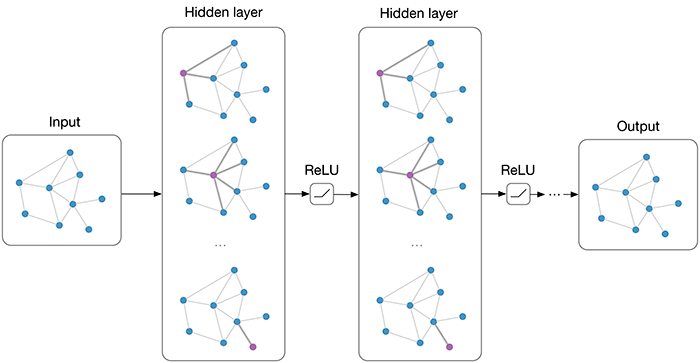
\includegraphics[width=0.8\textwidth]{images/20_material_methods/model.png}
    \caption{Modell für die Graphenklassifizierung (Quelle: \cite{kipf_semi-supervised_2017})}
    \label{fig:gcn_model}
\end{figure}

\newpage
\subsection{Unterschied von Graph-Embedding und Graph-Kernels}

Graph-Kernel-basierte Ansätze zersetzen einen Graphen in eine Menge von Subgraphen, Graphlets \cite{shervashidze_efficient_2009} oder Weisfeiler-Lehman-Kernels genannt \cite{shervashidze_weisfeiler-lehman_nodate}.
Diese Ansätze werden bisher verwendet, um die Ähnlichkeiten zwischen Graphen zu berechnen.
Beim Zersetzen von Graphen in Graph-Kernels geht es darum, möglichst viele Informationen auf ihre zentralen Merkmale zu reduzieren.
Diese Informationen werden dann in einem Vektor zusammengefasst und können mit anderen Vektoren verglichen werden.

Graph-Embedding ist ein Ansatz, welcher in den Graph Neural Networks verwendet wird. Der Ursprung geht auf William Hamilton und das Thema \enquote{Representation Learning} von Graphen zurück \cite{hamilton_inductive_2018}.
Die Aggregationsfunktion $ \phi $ ist ein Graph Neural Network, welches die Eigenschaften der Knoten in einen Vektor transformiert \cite{xu_how_2019}.
Mit der \textsc{ReadOut}-Funktion $ \rho $ werden die einzelnen Vektoren dann via Sum-Pooling zusammengefasst, um Graph-Embedding zu erhalten \cite{nguyen_universal_2022}.

\begin{figure}[H]
    \centering
    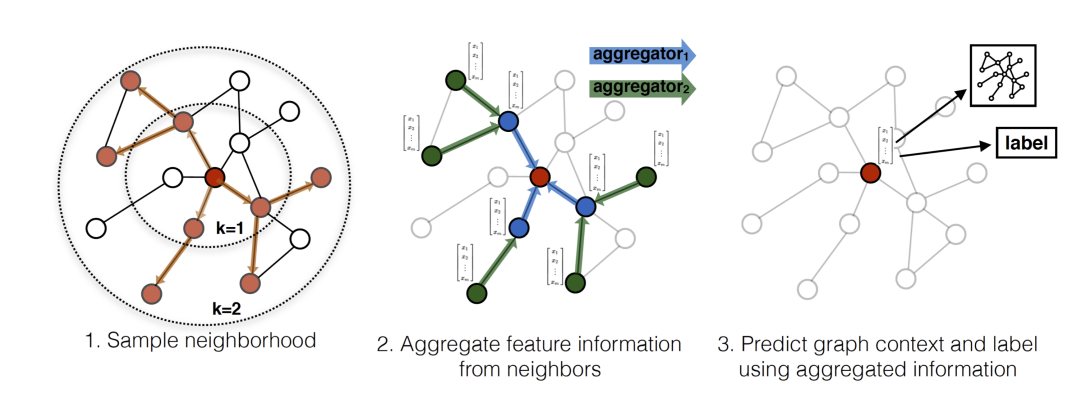
\includegraphics[width=9cm]{images/20_material_methods/graph_representation_learning.png}
    \caption{Sample- und Aggregation-Ansatz visualisiert (Quelle: Hamilton \cite{hamilton_inductive_2018})}
    \label{fig:graph_representation_learning}
\end{figure}

